% #############################################################################
% This is Chapter 5
% !TEX root = ../main.tex
% #############################################################################
% Change the Name of the Chapter i the following line
\fancychapter{Evaluation Setup}
\cleardoublepage
% The following line allows to ref this chapter
\label{chap:evaluation}

This chapter presents the experimental setup for evaluating open-vocabulary aerial image segmentation models. We describe the model architecture, training procedures, evaluation metrics, and baseline comparisons used in our study.

% #############################################################################
\section{Model Architecture}

Our approach is based on the RSRefSeg (Referring Segmentation with Rule-based annotation System) architecture, which combines text and visual understanding for precise object segmentation in aerial imagery.

\begin{figure}[H]
\centering
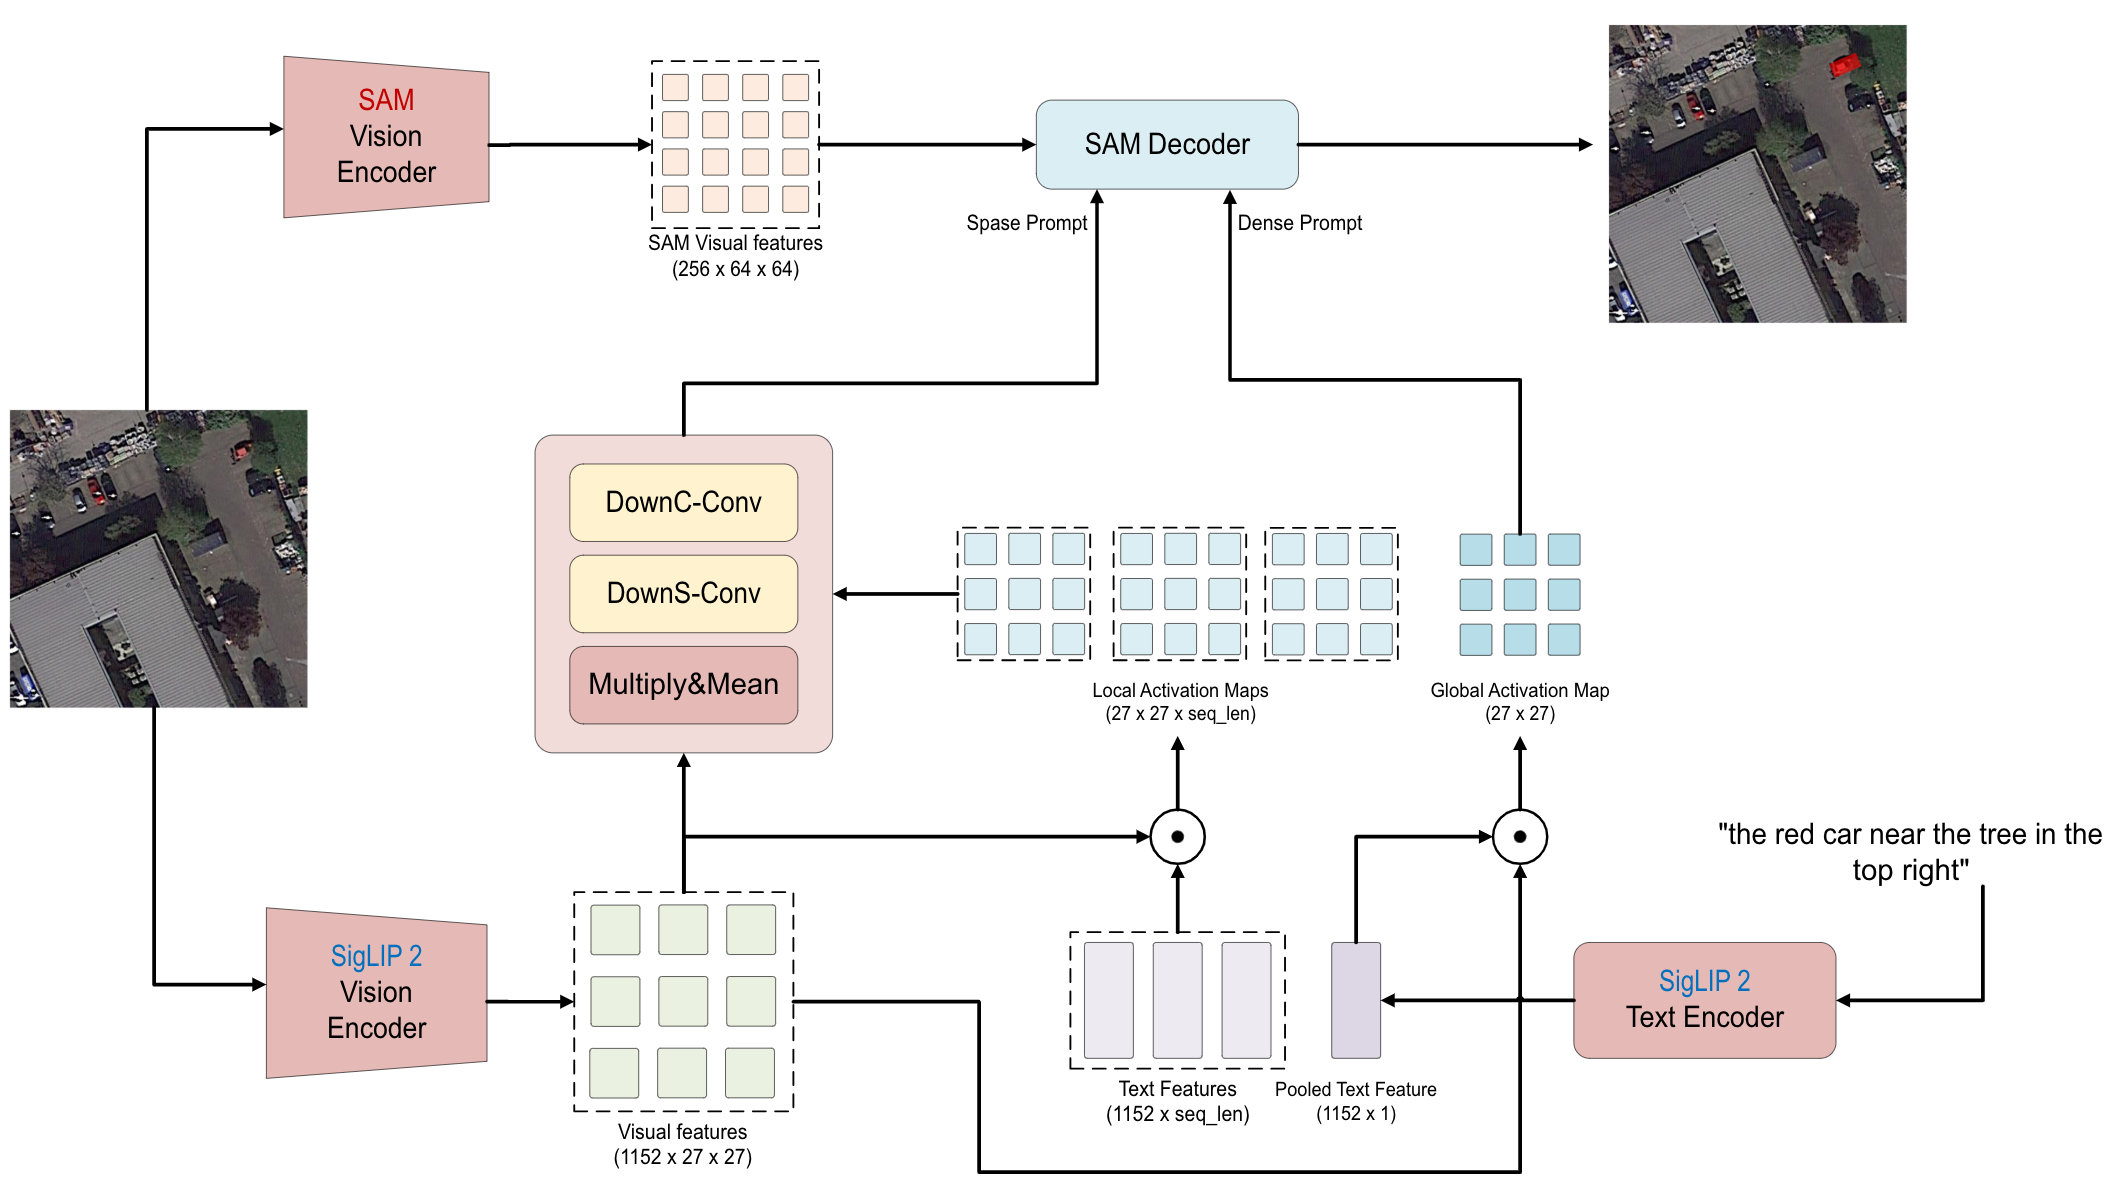
\includegraphics[width=\textwidth]{./Images/clipsam.png}
\caption{RSRefSeg architecture overview showing the integration of SigLIP2 vision-language encoder with SAM mask decoder through custom prompter networks for text-guided segmentation. The dual-pathway design processes both local (token-level) and global (sentence-level) text-visual interactions to generate sparse and dense prompts for precise aerial image segmentation.}
\label{fig:rsrefseg_architecture}
\end{figure}


% #############################################################################
\section{Experimental Configuration} 
This section describes the training configuration and experimental setup for evaluating the RSRefSeg model on the AerialD dataset.




\subsection{Training Configuration}

% [Training parameters, optimization settings, data splits, augmentation strategies, etc.]

\subsection{Evaluation Methodology}

% [Metrics, validation splits, cross-dataset testing, ablation study design, etc.]
